%%%%%%%%%%%%%%%%%%%%%%%%%%%%%%%%%%%%%%%%%%%%%%%%%%%%%%%%%%%%%%%%%%%%%%%%%%%%%%%%%
% ClapCap -- CENG416 A0 portrait poster.
% Base template: a0poster (CC BY-NC-SA 3.0, latextemplates.com), restyled to the
% 416A.tex report: Roboto sans + the audio-blue figure palette.
% Compile from reports/poster/ :  pdflatex clapcap_poster.tex
%%%%%%%%%%%%%%%%%%%%%%%%%%%%%%%%%%%%%%%%%%%%%%%%%%%%%%%%%%%%%%%%%%%%%%%%%%%%%%%%%

\documentclass[a0,portrait]{a0poster}

\usepackage{multicol}
\columnsep=80pt
\columnseprule=0pt

\usepackage[svgnames,table]{xcolor}
\usepackage[sfdefault]{roboto}     % Roboto sans, matching the 416A report
\usepackage[T1]{fontenc}
\usepackage{graphicx}
\graphicspath{{figures/}{../figures/}} % logo here; result PDFs in reports/figures/
\usepackage{booktabs}
\usepackage{array}
\usepackage[font=small,labelfont=bf]{caption}
\usepackage{amsfonts,amsmath,amssymb}
\usepackage{tikz}
\usetikzlibrary{arrows.meta,positioning}
\usepackage{tcolorbox}
\usepackage{enumitem}
\setlist[itemize]{leftmargin=1.4em,itemsep=4pt,topsep=4pt,parsep=0pt}
\setlist[enumerate]{leftmargin=1.6em,itemsep=4pt,topsep=4pt,parsep=0pt}
\usepackage{sectsty}
\sectionfont{\color{ccnavy}\fontsize{38}{46}\selectfont\bfseries}

% ---- palette lifted from the report figures -------------------------------
\definecolor{ccnavy}{HTML}{08306B}
\definecolor{ccblue}{HTML}{3182BD}
\definecolor{ccteal}{HTML}{1B8A6B}
\definecolor{ccwarm}{HTML}{C0392B}
\definecolor{ccink}{HTML}{2B2B2B}
\definecolor{cclight}{HTML}{EAF2FB}

\color{ccink}

% custom commands
\newcommand{\sys}{\textsc{ClapCap}}
\newcommand{\clapenc}{\textsc{Clap}}
\newcommand{\fense}{\textsc{Fense}}

\begin{document}

%--------------------------------------------------------------------- HEADER
\begin{minipage}[c]{0.16\linewidth}

\includegraphics[width=12cm]{iyte_logo.png}
\end{minipage}
\hspace{1cm}
\begin{minipage}[c]{0.66\linewidth}
\Huge \color{ccnavy}\textbf{ClapCap: CLAP Prefix for Music Captioning}\color{ccink}\\[0.4cm]
\Large A frozen \clapenc{} embedding $\rightarrow$ a short learned prefix $\rightarrow$ a small language model.\\[0.6cm]
\huge \textbf{Ali Ozkaya}\,\, (280201092)\\[0.3cm]
\Large Advisor: Prof.\ Dr.\ Aytu\u{g} Onan \quad\textbullet\quad Computer Engineering, Izmir Institute of Technology
\end{minipage}
\hspace{0.5cm}
\begin{minipage}[c]{0.14\linewidth}
\begin{tcolorbox}[colback=cclight,colframe=ccblue,boxrule=2pt,arc=6pt,left=6pt,right=6pt,top=6pt,bottom=6pt]
\centering\Large\color{ccnavy}\textbf{CENG416}\\[2mm]\large Senior Thesis\\Poster, 2026
\end{tcolorbox}
\end{minipage}

\vspace{0.5cm}
{\color{ccblue}\rule{\linewidth}{4pt}}
\vspace{0.3cm}

\begin{multicols}{2}

%--------------------------------------------------------------- SUMMARY
\section*{Summary}
\Large
\sys{} is the audio analogue of the ClipCap image-captioning recipe: a
\textbf{frozen} \clapenc{} audio encoder turns a 10\,s clip into one embedding, a
small projection MLP maps it to a fixed-length prefix of pseudo-tokens, and a
pretrained language model writes the caption. On MusicCaps we run a
\emph{controlled} comparison of two lightweight LM families --- GPT-2 (124M) and
T5-base (220M) --- holding encoder, projection, data split and evaluation fixed,
so the language model is the only variable.

\begin{tcolorbox}[colback=cclight,colframe=ccnavy,boxrule=2pt,arc=8pt]
\Large\textbf{One takeaway.} A \textbf{124M} frozen-prefix LM captions music
\emph{competitively with} dedicated music captioners and clearly beats the
clean ones on \fense{} --- one to two orders of magnitude smaller than
billion-parameter audio LLMs, trained on a \textbf{single consumer GPU}.
\end{tcolorbox}

%--------------------------------------------------------------- QUESTION
\section*{Research question}
\Large
\textit{Can a lightweight language model understand music semantics through a
simple projection from a frozen audio embedding?} And between two such models,
\emph{does the choice of LM matter} once run-to-run variance is accounted for?

%--------------------------------------------------------------- METHOD
\section*{Method: the \sys{} pipeline}
\vspace{0.3cm}
\begin{center}
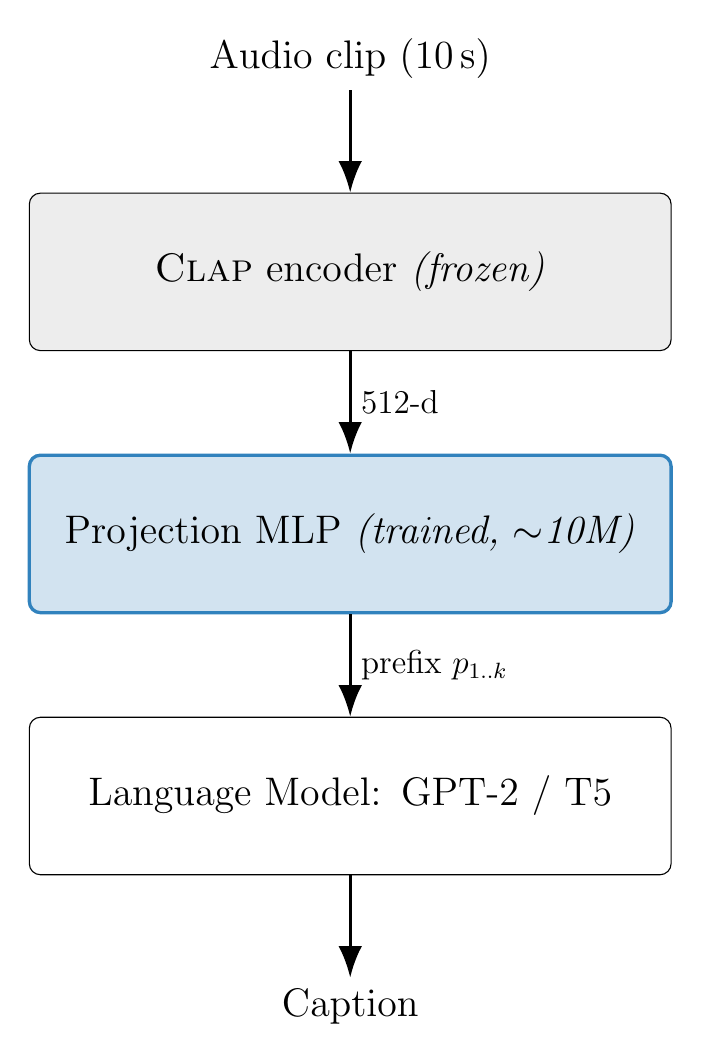
\begin{tikzpicture}[
    node distance=13mm,
    box/.style={draw, rounded corners, minimum height=20mm, text width=0.62\linewidth,
                align=center, inner sep=9pt, font=\Large},
    frozen/.style={box, fill=black!7},
    trained/.style={box, fill=ccblue!22, very thick, draw=ccblue},
    data/.style={align=center, font=\Large, inner sep=4pt},
    flow/.style={-{Latex[length=4mm]}, very thick}]
  \node[data] (audio) {Audio clip (10\,s)};
  \node[frozen, below=of audio] (clap) {\clapenc{} encoder \emph{(frozen)}};
  \node[trained, below=of clap] (proj) {Projection MLP \emph{(trained, $\sim$10M)}};
  \node[box, below=of proj] (lm) {Language Model: GPT-2 / T5};
  \node[data, below=of lm] (cap) {Caption};
  \draw[flow] (audio) -- (clap);
  \draw[flow] (clap) -- node[right,font=\large]{512-d} (proj);
  \draw[flow] (proj) -- node[right,font=\large]{prefix $p_{1..k}$} (lm);
  \draw[flow] (lm) -- (cap);
\end{tikzpicture}
\end{center}
\vspace{0.2cm}
\Large
\begin{itemize}
  \item \textbf{Only new module:} the projection MLP ($\sim$10.2M params);
        \clapenc{} embeddings are precomputed once, so the encoder never runs in training.
  \item \textbf{Two-stage training:} Stage 1 trains the projection with the LM
        frozen; Stage 2 also fine-tunes the LM.
  \item \textbf{Evaluation:} a ten-metric suite with \fense{} as the primary
        score; a per-model \emph{noise floor} from three seeds, so every ablation
        delta is judged against run-to-run variance.
\end{itemize}

%--------------------------------------------------------------- RESULTS 1
\section*{Result 1 --- vs.\ reference captioners}
\Large
On the shared MusicCaps test split the \sys{} best-decoding rows
(GPT-2 \fense{} \textbf{0.580}, T5 \textbf{0.576}) \emph{outscore every clean
reference captioner} --- music-domain (LP-MusicCaps pretrain 0.378; BLAP 0.476,
held-out) and general-audio (NVIDIA Audio Flamingo, Qwen2-Audio, Qwen3-Omni)
alike. Rows marked $\dagger$ may have seen MusicCaps in training, so their bars
are leakage upper bounds, not clean held-out scores.
\begin{center}
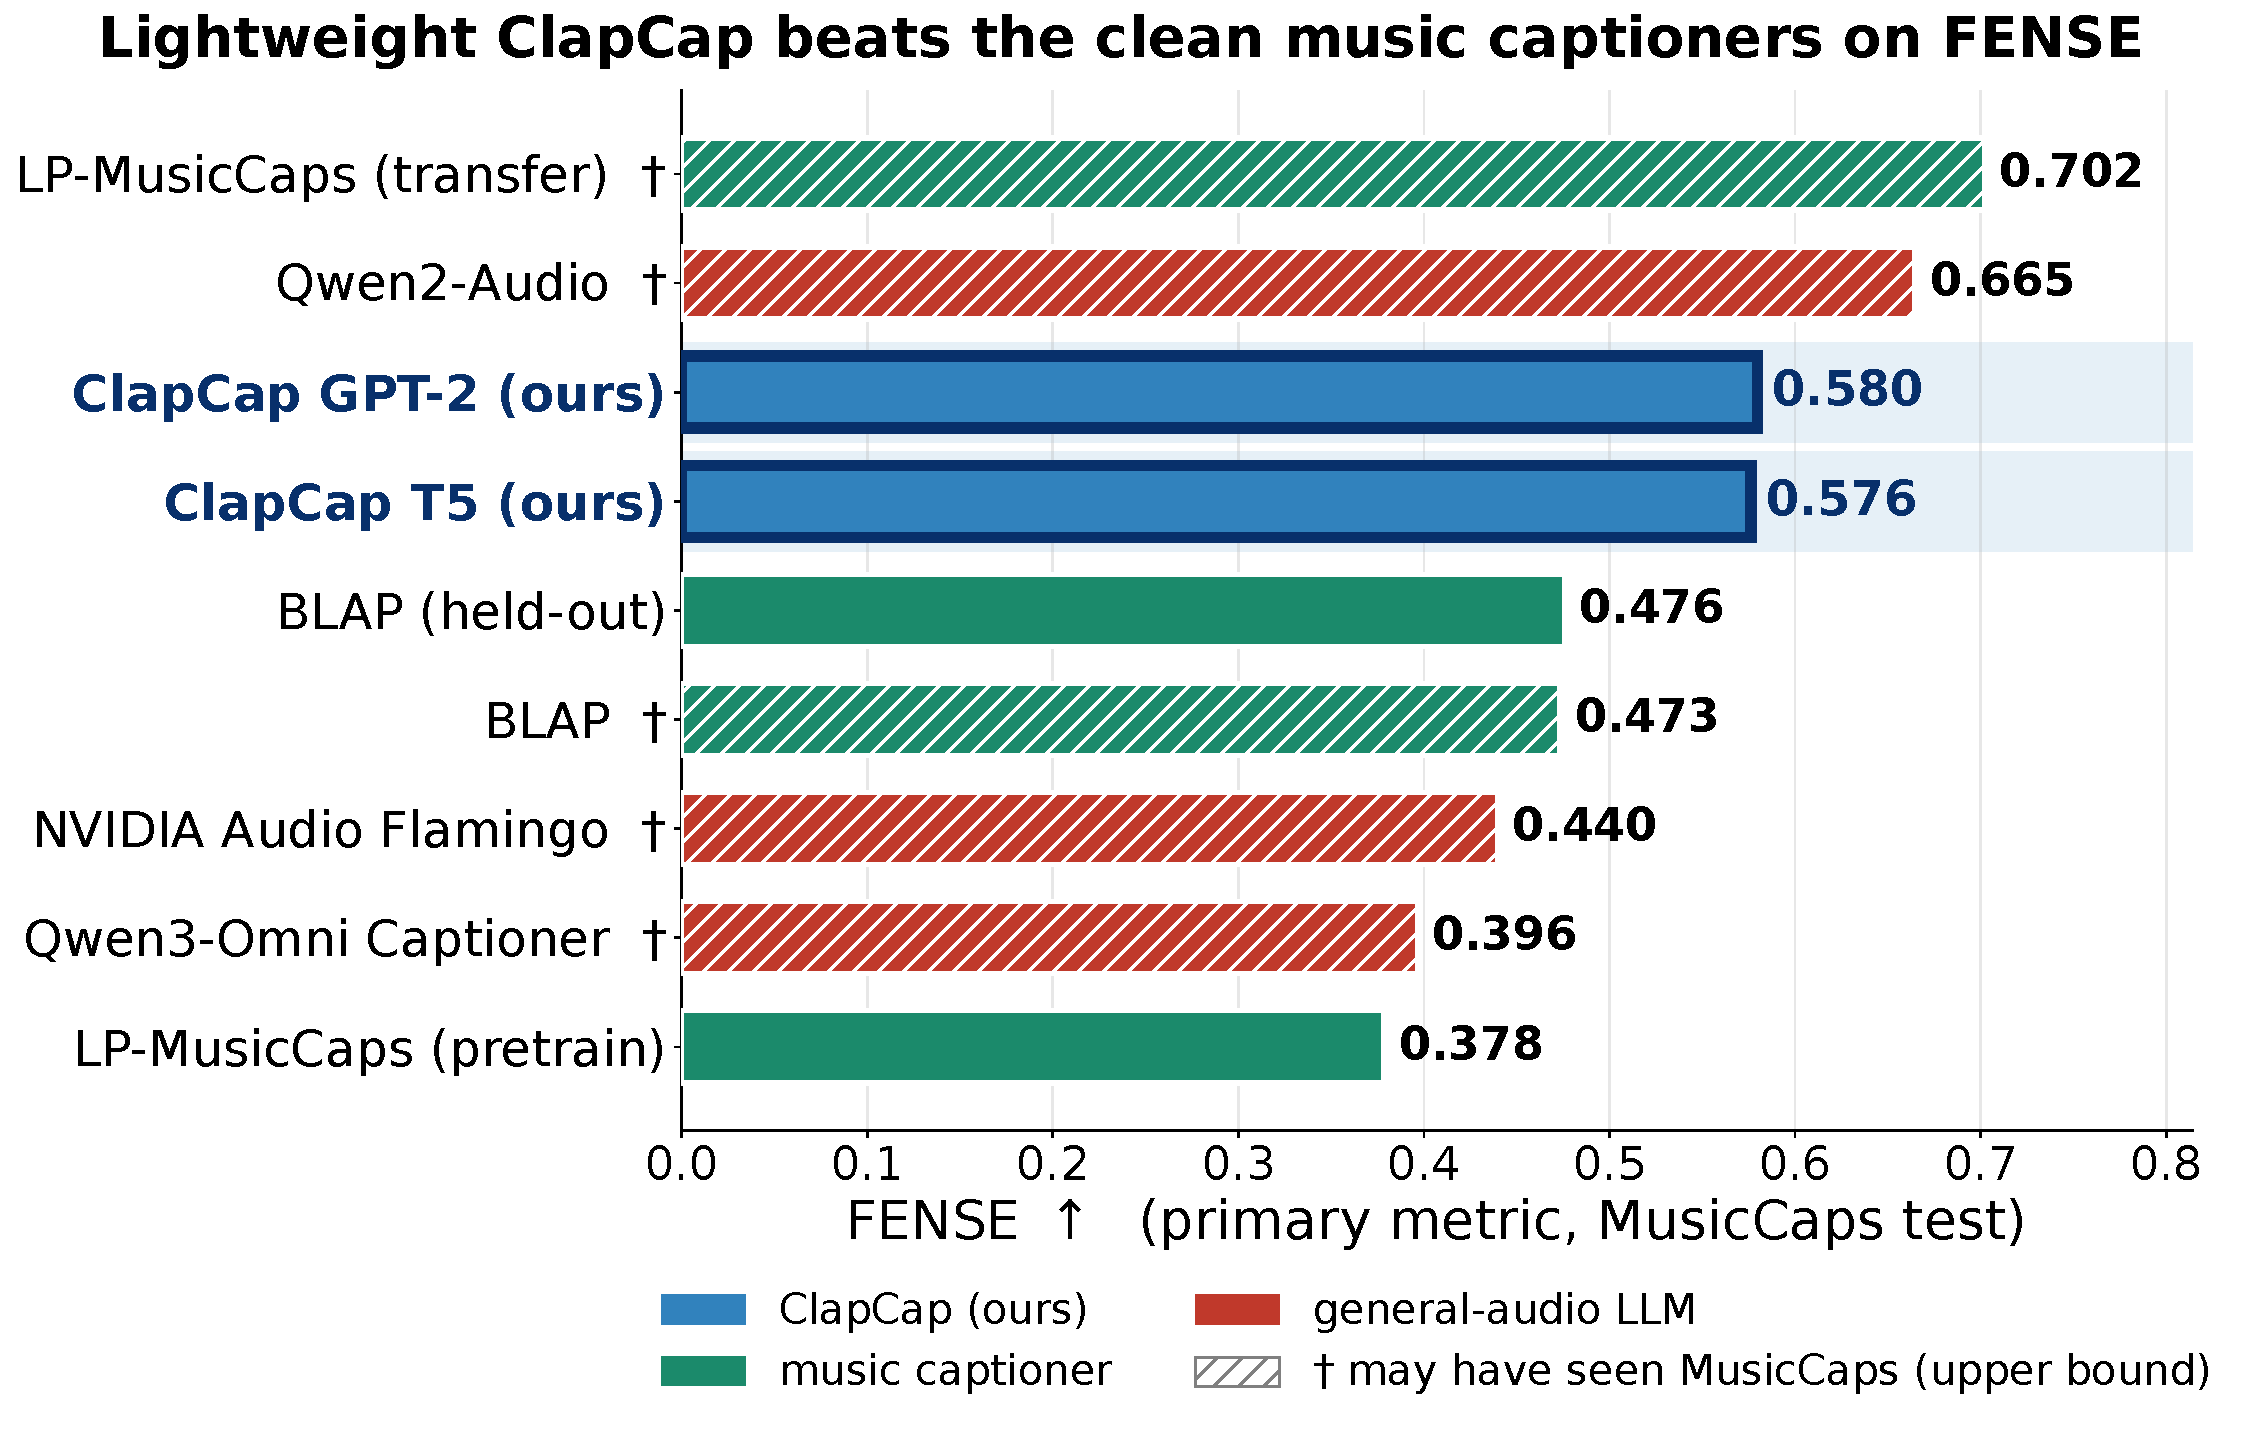
\includegraphics[width=\linewidth]{fig_poster_fense.pdf}
\end{center}

%--------------------------------------------------------------- RESULTS 2
\section*{Result 2 --- pairwise A/B evaluation}
\Large
A pairwise A/B study (more accurate? / less wrong?) across \textbf{three rater
pools} --- 10 human listeners, 3 audio LLM judges, 5 text LLM judges. Every pool
\textbf{prefers GPT-2-best over T5-best}; the \textbf{reference still wins}, the
honest ceiling. Lay humans are noisy individually (Fleiss $\kappa$ 0.13) but their
\emph{consensus} tracks the audio panel (human$\leftrightarrow$LLM $\kappa = 0.64$).
\vspace{0.5cm}
\begin{center}
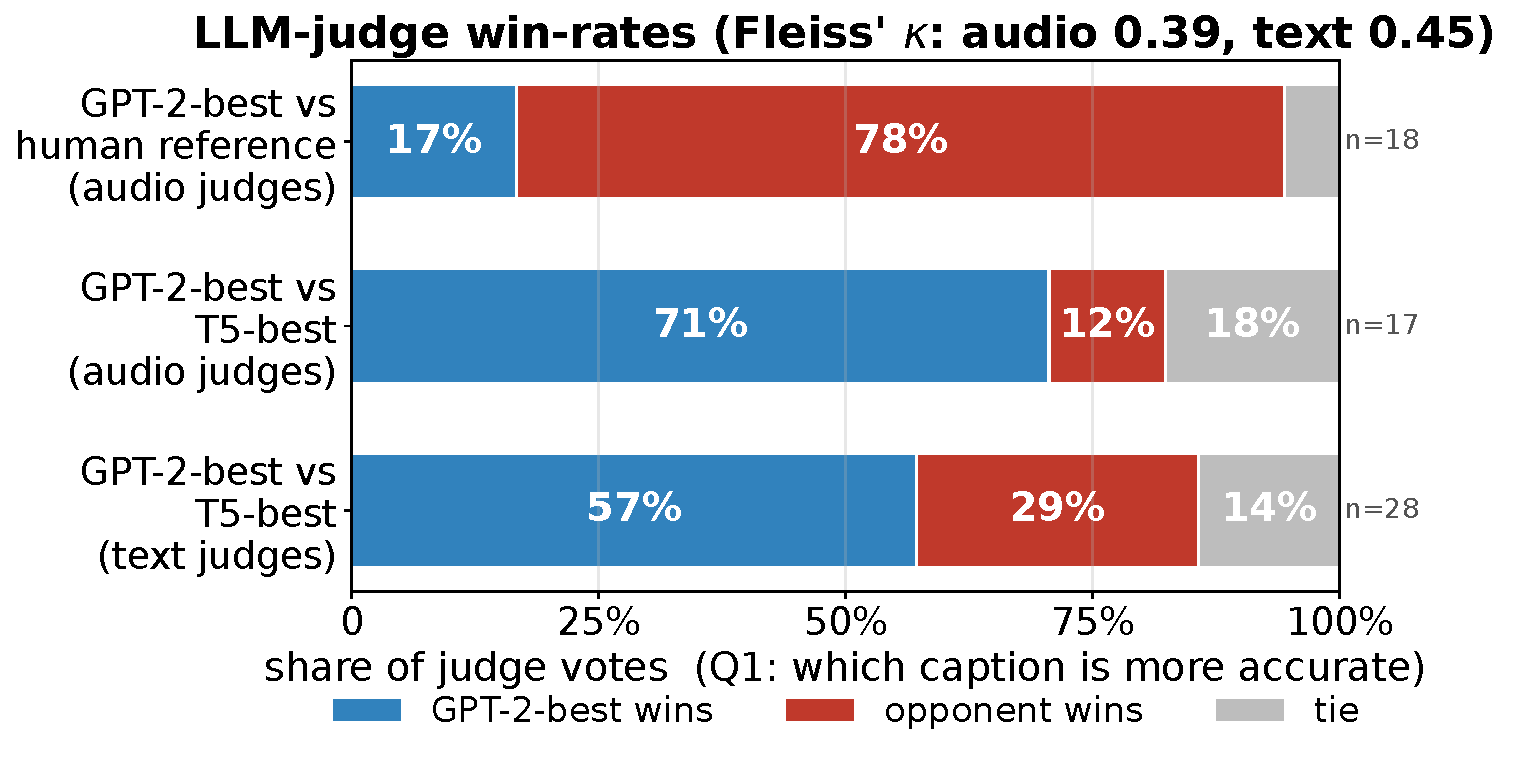
\includegraphics[width=\linewidth]{fig_eval_winrate.pdf}
\end{center}

%--------------------------------------------------------------- FINDINGS
\section*{Key findings}
\Large
\begin{enumerate}
  \item GPT-2 and T5 are \textbf{statistically indistinguishable at baseline}
        once the noise floor is accounted for.
  \item Stage-2 fine-tuning \textbf{erases} nearly all architectural differences
        introduced in the projection stage.
  \item The largest decoding lever (sentence completion) lifts \fense{} mainly by
        \textbf{removing fluency errors}, not by adding semantic content.
  \item Lightweight, single-GPU \sys{} is \textbf{competitive} with dedicated
        music captioners --- the recipe, not scale, carries the result.
\end{enumerate}

%--------------------------------------------------------------- CONCLUSION
\section*{Conclusion}
\Large
A frozen audio embedding plus a short learned prefix is enough for a 124M LM to
describe music. The controlled analysis --- and the efficiency of the recipe ---
is the contribution, not a single leaderboard number.

{\normalsize\color{ccink}
\textbf{Acknowledgements.} Advisor Prof.\ Dr.\ Aytu\u{g} Onan. Built on
ClipCap (Mokady et al.\ 2021) and \clapenc{} (Wu et al.\ 2023); evaluated with
the \fense{} and aac-metrics suites on MusicCaps. Single NVIDIA RTX~5090.}

\end{multicols}
\end{document}
